\documentclass{conception_detaillee}
\usepackage{lipsum}
\usepackage{hyperref}
\usepackage{enumitem}
\usepackage{titlesec}
\usepackage{geometry}
\usepackage{longtable}
\titleformat{\section}{\large\bfseries}{\thesection}{1em}{}
\titleformat{\subsection}{\normalsize\bfseries}{\hspace{1em}\thesubsection}{1em}{}
\titleformat{\subsubsection}{\small\bfseries}{\hspace{2em}\thesubsubsection}{1em}{}
\title{Cahier de recette - L2I1} %Titre du fichier

\begin{document}

%----------- Informations du rapport ---------

\titre{Conception détaillée \\ L2I1 - Tamagotchi} %Titre du fichier .pdf
\UE{UE Projet de programmation} %Nom de la UE
\sujet{Projet L2I1 - Tamagotchi} %Nom du sujet

\encadrant{Camille \textsc{KURTZ}} %Nom de l'enseignant
\responsable{David \textsc{JANISZEK}}

\auteurs{Marwan \textsc{DENAGNON} \\
		Lina \textsc{BOUGUETTAYA} \\ 
		Yasmine \textsc{DEHOUCHE} \\
		Abhijeet \textsc{SINGH}} %Nom des élèves

%----------- Initialisation -------------------
        
\fairemarges %Afficher les marges
\fairepagedegarde %Créer la page de garde
\renewcommand{\contentsname}{Sommaire}
\tableofcontents %Créer la table de matières
\newpage


%------------ Corps du rapport ----------------


\section{Introduction} 

Ce document constitue \textbf{la conception détaillée} de notre projet de programmation L2I1: Simulation de vie d’un petit animal. 
Cette \textbf{conception détaillée} a pour objectif de définir, formaliser et expliquer les aspects techniques tout en permettant de vérifier et d’indiquer l’architecture de l’application. On y trouve la définition des différentes fonctions, classes, librairie et autres structures dont on a besoin pour développer cette application.
Ce document contiendra plusieurs parties, nous désignons d’abord les objectifs de base à la compréhension de notre projet, ensuite nous enchaînons avec l’architecture de logicielle, ainsi que les technologies et outils qui seront utilisées lors de l’étape de  développement, nous y trouvons également la partie planification et l’organisation des tâches qui est primordiale pour la fluidité et structuration de cette phase de développement. Elle contient également la schématisation des structures prête à ce que celà soit facilement traduit en code source. 
Ce document servira de référence tout au long du développement du projet afin d’assurer une conception structurée et rigoureuse.

\subsection{Objectifs et méthodes}
Notre objectif primaire est de créer une application android fonctionnelle pour prendre soin d’un animal de compagnie virtuel, voire deux. Ce dernier sera nourri, lavé, diverti et soigné pour répondre à ses besoins afin de le garder en vie. Si le maître de l’animal n’est pas disponible pour cela, nous prévenons un système NFC pour transférer la créature à quelqu'un qui pourra s’en occuper entre temps. Le contenu de ce document nous permettra de mettre un doigt sur les détails de conception techniques.
\subsection{Documents de référence}
Les documents de référence de ce projet sont: 
\begin{itemize}[label=\textbullet]
\item Le descriptif du projet.
\item https://www.ens.math-info.univ-paris5.fr/projets-informatiques/doku.php?id=projets:licence2:2024-2025
\item Le cahier des charges.
\item Le cahier de recette
\item La maquette de l’application
\item Les comptes rendus de chaque réunion. 

\section{Guide de lecture}

\subsection{Maîtrise d’œuvre}
\subsubsection{Responsable}
Nom de l'encadrant : Kurtz Camille 

Le maître d'œuvre supervise et apporte un soutien aux propositions de l’équipe concernant le développement de l’application android. Il s’occupe de la validation des documents principaux. 
\subsubsection{Personnel technique}
Le personnel du projet est constitué des quatres étudiants choisie: 
\begin{itemize}[label=\textbullet]
\item Lina BOUGUETTAYA 
\item Yasmine DEHOUCHE
\item Marwan DENAGNON 
\item Abhijeet SINGH
\end{itemize}
\subsection{Maîtrise d'ouvrage}
Le maître d’ouvrage est le client de notre projet. Ce dernier est représenté par l’encadrant du groupe M. KURTZ. 
\section{Architecture logiciel}
L'architecture est basée sur MVVM (Model-View-ViewModel), un modèle populaire dans les applications Android modernes, qui permet une séparation claire des responsabilités tout en facilitant la gestion de l'état de l'application.
\begin{itemize}[label=\textbullet]
\item Model : Représente les données de l'application et la logique métier.
\item View : Gère l'interface utilisateur (UI).
\item ViewModel : Gère les interactions entre la View et le Model, et contient la logique de présentation.
\end{itemize}
\section{Technologies et outils}
\subsection{Front end}
Utilise des outils et
technologies qui permettent la modélisation de l’application :
\begin{itemize}[label=\textbullet]
\item Figma : outil de conception visuelle utilisé pour la
réalisation de maquettes interactives de l’interface
utilisateur.
\item Canva : plateforme graphique utilisée pour la création d’assets graphiques destinés à l’application.
\item XML (Extensible Markup Language) : langage de balisage utilisé pour structurer, stocker et échanger les données de manière hiérarchique.
\end{itemize}
\subsection{Back end}
Repose sur un ensemble
d’outils afin d’assurer la gestion et l’interaction avec
l’interface utilisateur :
\begin{itemize}[label=\textbullet]
\item Android Studio : environnement de développement
intégré officiel pour Android ayan des outils avancés
pour l’édition du code, le débogage et l’émulation
de l’application.
\item Java : langage de programmation utilisé pour
implémenter les fonctionnalités de l’application.
\item Android SDK : Ensemble d’outils fournis par google
pour le développement d’applications Android.
\item JSON (JavaScript Object Notation) : représentation
structurée des données sous forme de paires clé-valeur, utilisée pour échanger des informations
entre un client et un serveur.
\end{itemize}
\subsection{Gestion de version et collaboration}
Se base sur des
outils permettant une coordination fluide entre les
membres de l’équipe afin de garantir la qualité du code
tout au long du développement :
\begin{itemize}[label=\textbullet]
\item Apache Subversion (SVN) : système permettant le
suivi des modifications du code source et la
collaboration entre les membres de l’équipe.
\item GitHub : plateforme de gestion et de collaboration
permettant l’hébergement du code source
\end{itemize}
\section{Description des modules}
\subsection{Page de choix de connexion ou d'inscription}
\begin{itemize}
    \item Bouton \textbf{“Se créer un compte”}
    \item Bouton \textbf{“J’ai déjà un compte”}
\end{itemize}

\subsection{Page de connexion}
\begin{itemize}
    \item Champs \textbf{Identifiant} et \textbf{Mot de Passe}
    \item Bouton \textbf{“Connexion”}
\end{itemize}

\subsection{Page d’inscription}
\begin{itemize}
    \item Champs \textbf{Nom} et \textbf{Prénom}
    \item Champ \textbf{Date de naissance}
    \item Champ \textbf{Genre de l’animal}
    \item Bouton \textbf{“S'inscrire”}
\end{itemize}

\subsection{Page de chargement}
\begin{itemize}
    \item Barre de chargement
\end{itemize}

\subsection{Page d’accueil}
\begin{itemize}
    \item Barre d'état de l’animal
    \item Bulle de discussion \textbf{“Salut”}
    \item Barre de tâches \textbf{“Soigner, Manger...”}
\end{itemize}

\subsection{Page d'information de l’animal et de l'utilisateur}
\begin{itemize}
    \item Fiche d'information concernant l’animal et son maître
    \item Champ du \textbf{Nom de l’animal} (possibilité de le changer)
    \item Bouton de \textbf{Paramètres}
\end{itemize}

\subsection{Page de paramètres}
\begin{itemize}
    \item Switch de synchronisation NFC
    \item Switch de désactivation des effets sonores
    \item Switch de désactivation des animations
    \item Switch \textbf{“Ajout d’un widget à l’écran d'accueil”}
    \item Bouton de \textbf{Déconnexion}
\end{itemize}

\subsection{Page de transfert NFC}
\begin{itemize}
    \item Bouton de confirmation \textbf{“Transférer vos données”}
\end{itemize}

\subsection{Page de gestion des données}
\begin{itemize}
    \item Création ou téléchargement d’un \textbf{Backup local}
    \item Exportation des données
    \item Bouton \textbf{Suppression des données}
\end{itemize}

\subsection{Page d’états de l’animal}
\subsubsection{État de faim}
\begin{itemize}
    \item Bulle de discussion \textbf{“J’ai faim”}
    \item Diminution de la barre de \textbf{Nourriture}
\end{itemize}

\subsubsection{État de saleté}
\begin{itemize}
    \item Bulle de discussion \textbf{“Je veux un bain”}
    \item Diminution de la barre de \textbf{Propreté}
    \item Affichage d’un animal sale
\end{itemize}

\subsubsection{État d’ennui}
\begin{itemize}
    \item Bulle de discussion \textbf{“Je m’ennuie ! joue avec moi”}
    \item Diminution de la barre de \textbf{Loisir}
    \item Affichage d’un animal qui s'ennuie
\end{itemize}

\subsubsection{État de sommeil}
\begin{itemize}
    \item Bulle de discussion \textbf{“Je veux dormir”}
    \item Diminution de la barre de \textbf{Sommeil}
    \item Affichage d’un animal fatigué
\end{itemize}

\subsubsection{État de maladie}
\begin{itemize}
    \item Bulle de discussion \textbf{“J’ai bobo”}
    \item Diminution de la barre de \textbf{Santé}
    \item Affichage d’un animal malade
\end{itemize}

\subsubsection{État de soif}
\begin{itemize}
    \item Bulle de discussion \textbf{“J’ai soif !”}
    \item Diminution de la barre de \textbf{Soif}
    \item Affichage d’un animal qui a soif
\end{itemize}

\subsubsection{État de négligence}
\begin{itemize}
    \item Bulle de discussion \textbf{“Je me sens délaissé! prends soin de moi”}
    \item Diminution de toutes les barres d’états
    \item Affichage d’un animal en mauvaise mine
\end{itemize}

\subsubsection{État de mort}
\begin{itemize}
    \item Toutes les barres sont à zéro
    \item Affichage d’un animal mort
\end{itemize}
\section{Arborescence de l'application}
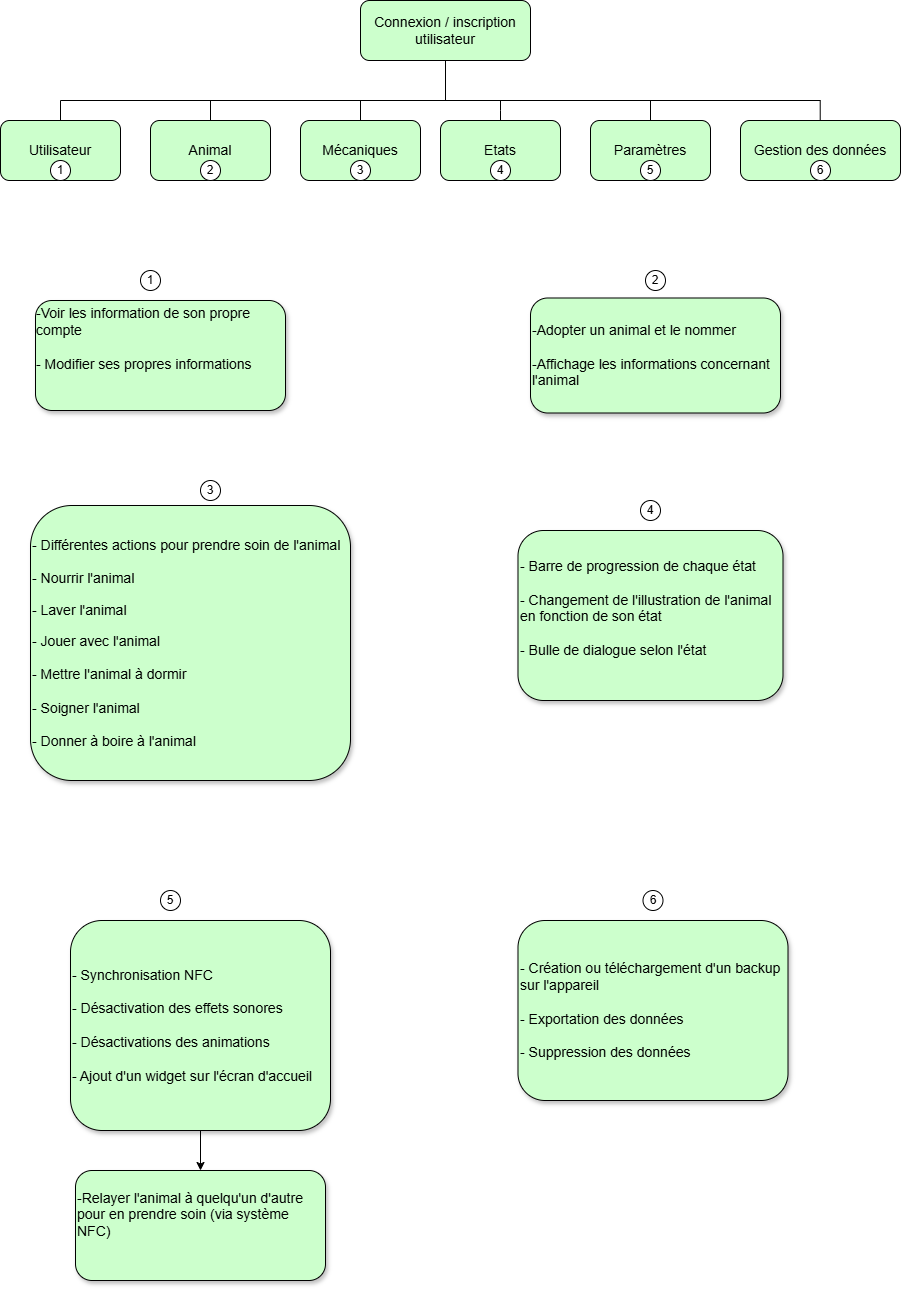
\includegraphics[height=0.8\paperheight]{images/ArborescenceL2i1.png}
\section{Diagramme de cas d'utilisation}
\noindent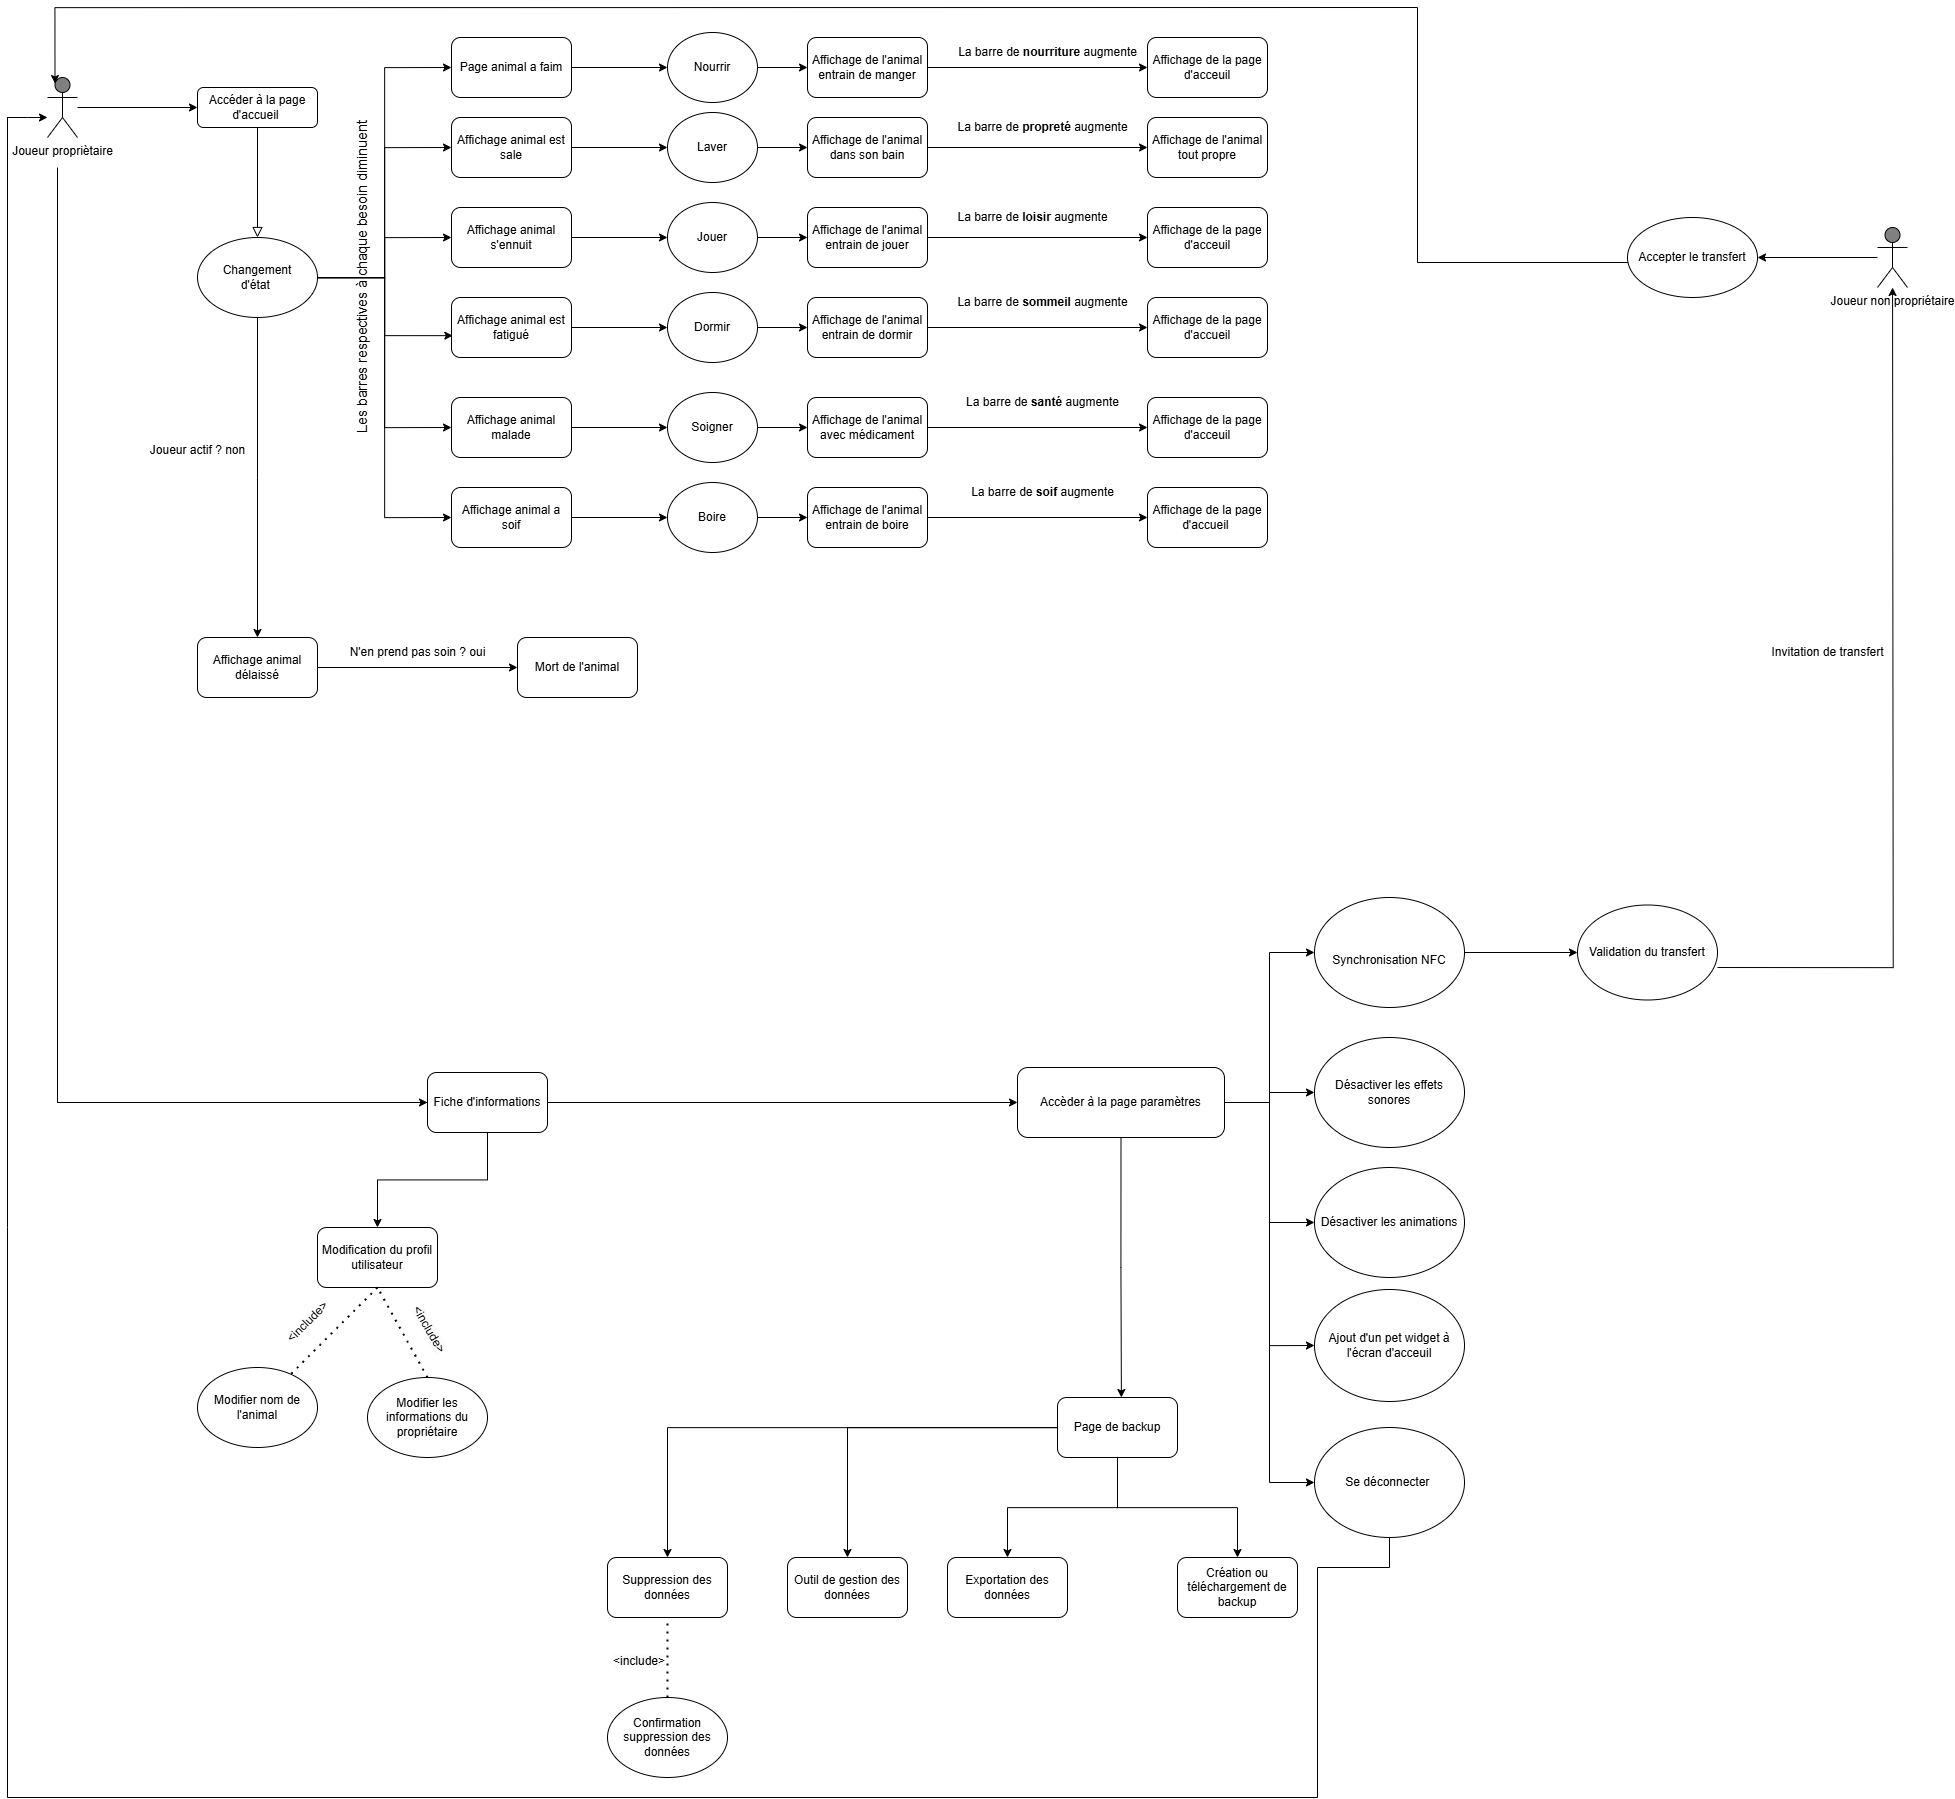
\includegraphics[width=0.8\paperwidth, height=0.8\paperheight]{images/utilisation.png}
\subsection{Diagramme de connexion}
\noindent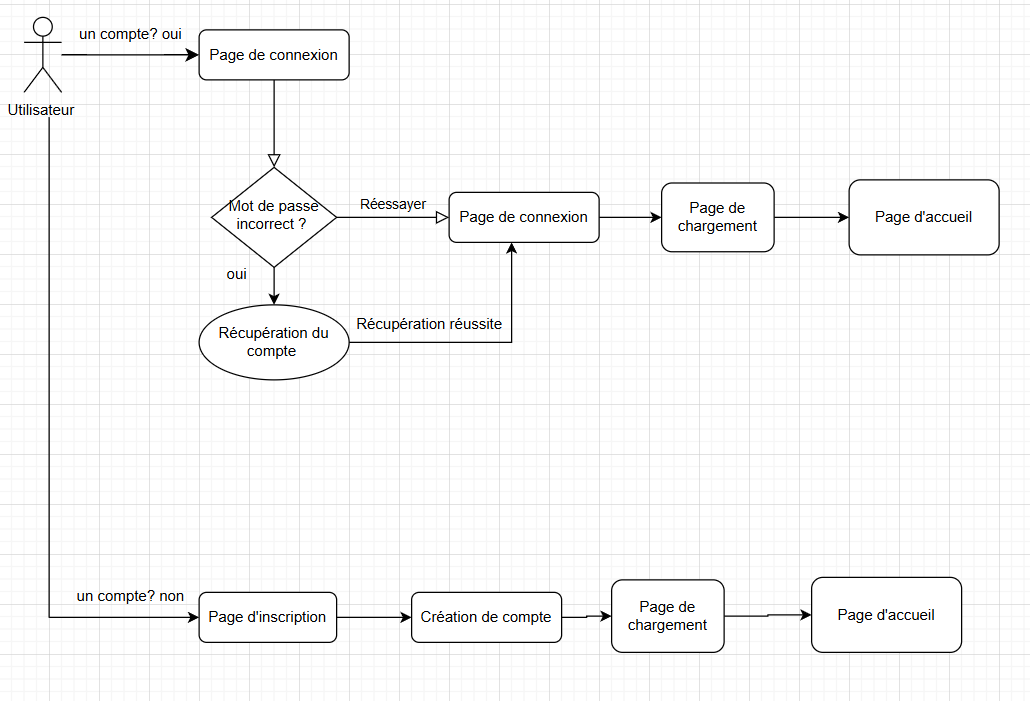
\includegraphics[width=0.8\paperwidth]{images/connexion.png}
\section{Diagramme de classes}
Les getters et setters qui ne font qu'une simple lecture/écriture ne sont pas inclus.
\noindent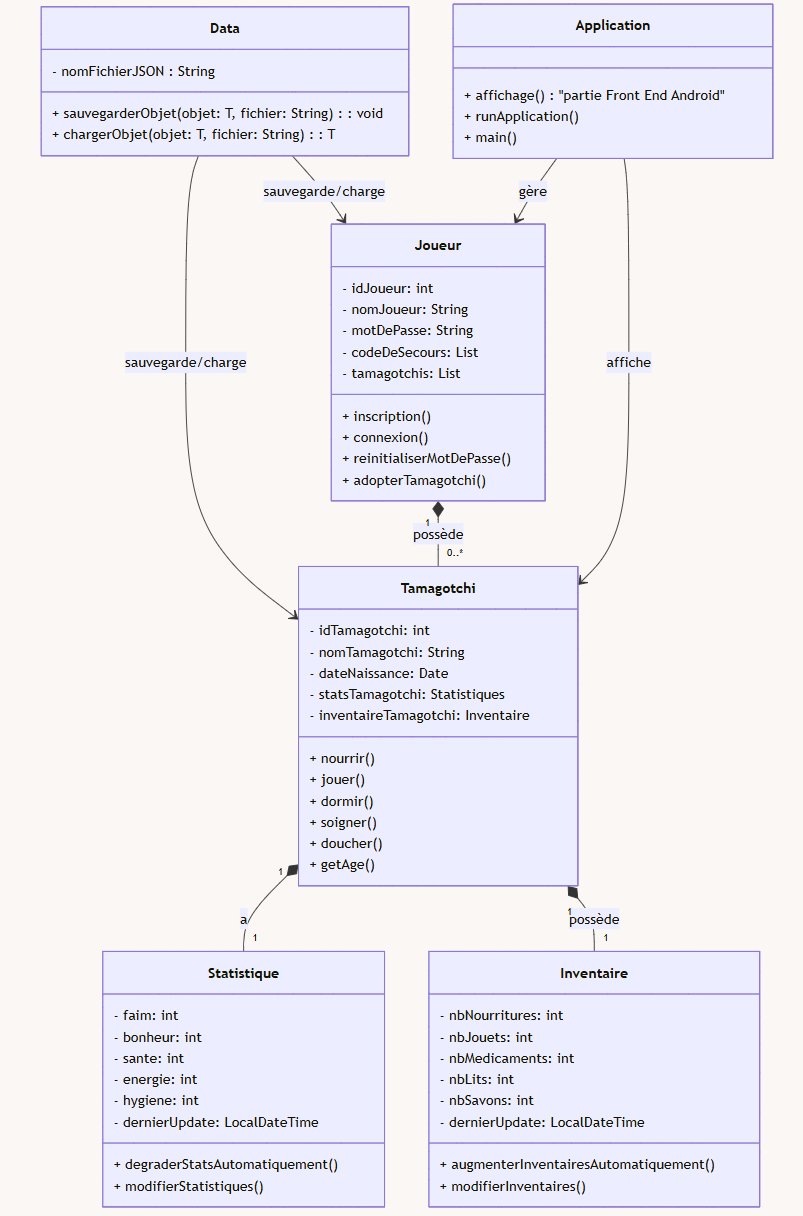
\includegraphics[width=0.8\paperwidth, height=0.8\paperheight]{images/diagramme_classe.png}
\section{Conception de la base de données (Modèle ERD)}
\noindent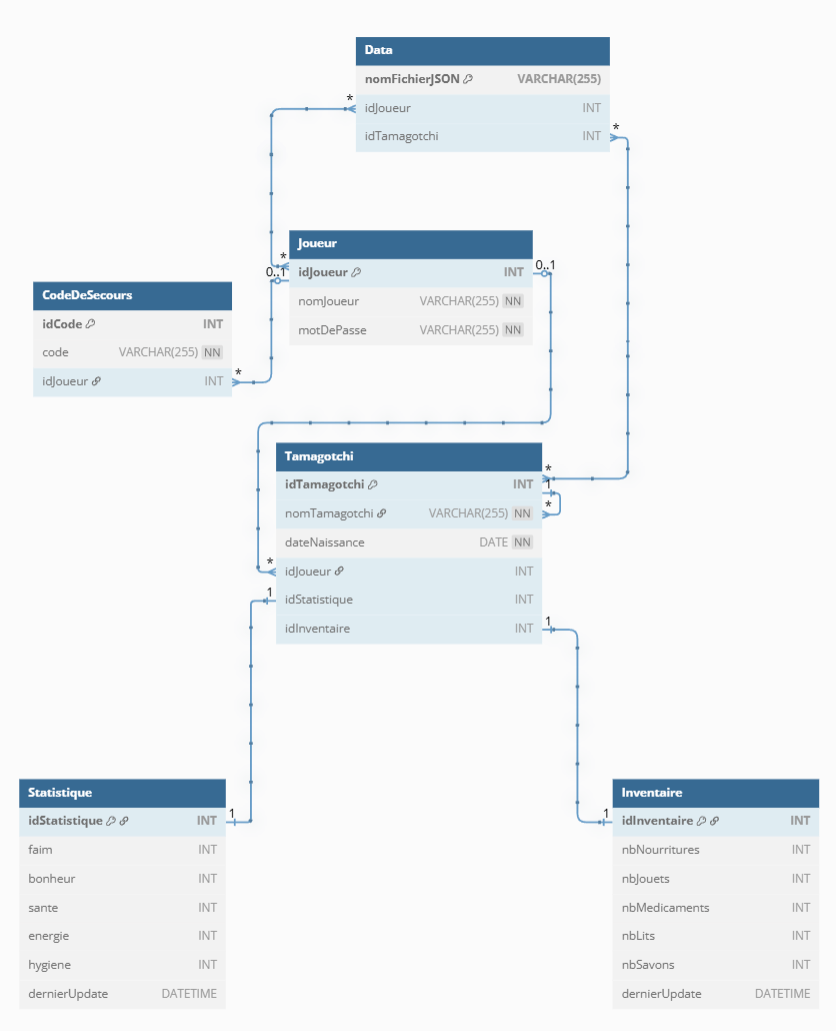
\includegraphics{images/erd2.png}
\section{Diagramme: Cycle de vie}
Le cycle de vie d’un projet décrit l’ensemble des processus nécessaires à sa
réalisation. Il se compose de différentes étapes, illustrées par le schéma général
ci-dessous :
\noindent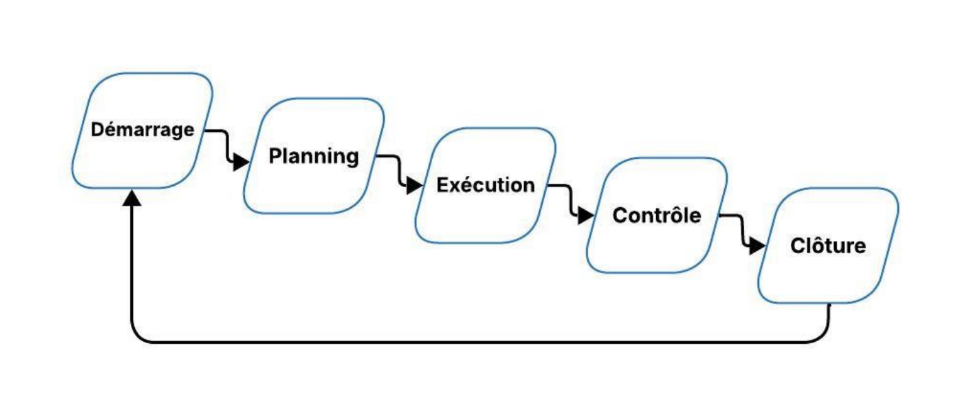
\includegraphics[width=0.8\paperwidth]{images/cycle_de_vie.png}
\textbf{Démarrage (initialisation)} : identification des besoins et validation du
lancement du projet.\\
\textbf{Planning} : précision des objectifs et organisation des tâches, des ressources et des délais nécessaires.\\
\textbf{Exécution} : réalisation du travail défini précédemment pour atteindre les
objectifs.\\
\textbf{Contrôle (surveillance)} : vérification de l’avancement et ajustement des écarts
si nécessaire.\\
\textbf{Clôture} : finalisation du projet, évaluation des résultats et archivage des
documents.
\newpage
\section{Organisation}
Le tableau ci-dessous représente l’organisation du projet sous forme de
décomposition des tâches :
\begin{table}[h]
    \centering
    \renewcommand{\arraystretch}{1.3}
    \begin{tabular}{|c|p{12cm}|}
        \hline
        \textbf{Id} & \textbf{Tâche} \\
        \hline
        1 & \textbf{Développement Frontend} des pages principales de l’application : \newline 
        - Création de maquettes pour l’interface utilisateur (UI) ; \\
        \hline
        2 & \textbf{Développement Frontend} : \newline
        - Implémentation de l’UI (boutons, états, actions) ; \\
        \hline
        3 & \textbf{Développement Backend} : \newline
        - Implémentation de la création et de la gestion de l’animal (interactions et états) ; \\
        \hline
        4 & \textbf{Développement Backend} : \newline
        - Création et gestion de la base de données pour stockage ; \\
        \hline
        5 & \textbf{Développement Frontend} : \newline
        - Implémentation des animations de l’animal ; \\
        \hline
        6 & \textbf{Développement Backend et Frontend} : \newline
        - Intégration des fonctionnalités en reliant le Backend aux éléments du Frontend ; \\
        \hline
        7 & \textbf{Développement Backend et Frontend} : \newline
        - Tests unitaires des fonctionnalités et débogage si nécessaire ; \\
        \hline
        8 & \textbf{Développement Backend et Frontend} : \newline
        - Tests finaux après débogage et optimisation ; \\
        \hline
        9 & \textbf{Développement Backend et Frontend} : \newline
        - Préparation de l’application pour déploiement et lancement ; \\
        \hline
    \end{tabular}
    \caption{Organisation des tâches du projet}
    \label{tab:organisation}
\end{table}
\section{Planification}
\subsection{Planning des projets}
Le projet s’étend sur une période de 12 semaines, ponctuée de réunions
hebdomadaires. Il se conclut par des soutenances et la remise d’un rapport. Les
quatre premières semaines sont consacrées à la documentation, comprenant la
rédaction du cahier des charges, du cahier de recettes et du plan de tests. Les
six semaines suivantes sont dédiées au développement. Enfin, les deux
dernières semaines seront réservées à la rédaction du rapport et à la
préparation de la soutenance.
Le diagramme ci-dessous montre la répartition des tâches sur la durée du
projet :\\
\noindent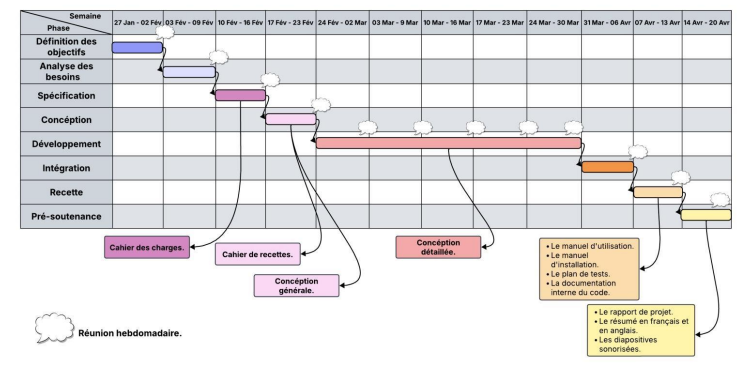
\includegraphics{images/gantt.png}
\subsection{Diagramme de Gantt de la planification}
\noindent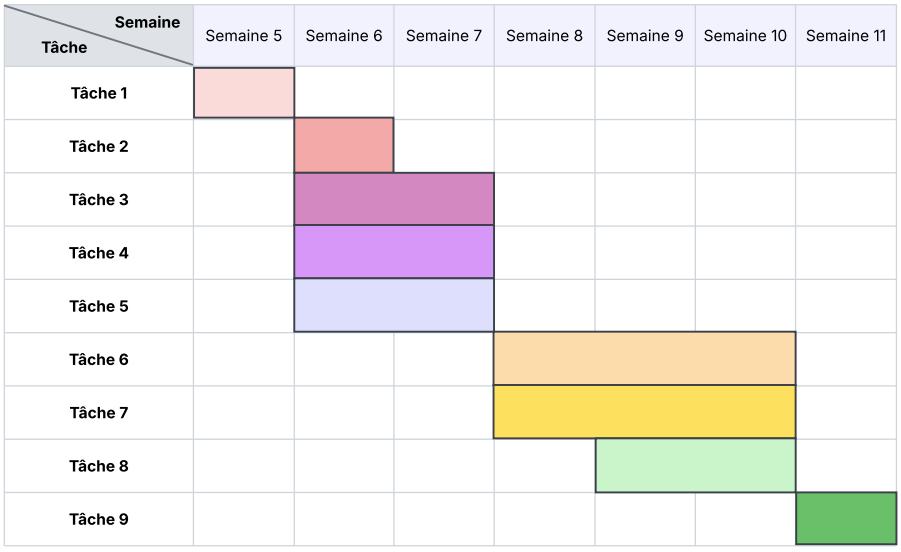
\includegraphics[width=0.8\paperwidth]{images/gantt2.png}
\section{Glossaire}
\begin{itemize}[label=\textbullet]
\item Arborescence: Structure hiérarchique représentant l'organisation ou la disposition des éléments dans un système.
\item Diagramme :Représentation visuelle utilisée pour illustrer des concepts, des processus ou des relations entre des éléments.
\item Diagramme de Gantt: Outil de gestion de projet utilisé pour planifier et suivre les tâches d’un projet dans le temps
\item Front-end : Partie visible d'un site ou d'une application avec laquelle l'utilisateur interagit ici tous ce qui est visible sur l'application.
\item Back-end : Partie cachée qui gère la logique, les bases de données et le serveur, ici le fichier JSON
\item Joueur non propriétaire: C'est l'utilisateur de l'appareil auquel le transfert sera fait pour s'occuper de l'animal lors de l'absence du maitre
\end{itemize}
\end{document}